\usepackage[authoryear,round]{natbib}
\usepackage{multirow}

\newcommand{\sheetnum}{%
	01
}
%\setcounter{section}{\sheetnum-3}
\newcommand{\tutorialtitle}{%
    Principal Component Analysis
}
\newcommand{\tutorialtitleshort}{%
	PCA
}
% for slides
\subtitle{\sheetnum \tutorialtitle}

%\maxdeadcycles=1000 % Workaround for ! Output loop---100 consecutive dead cycles because of too many figures

% The following use of algroithms does not work well with the notes:
%
%
%
%
% instead use the following for your algorithms:
%
%\begin{figure}[!t]
%\removelatexerror
%\begin{algorithm}[H]
    % your algo here
    %\label{alg:algolabel}
    %\caption{algocaption}
%\end{algorithm}
%\end{figure}
%\begin{algorithm}
% Below is the definition for the command \removelatexerror:
\makeatletter
\newcommand{\removelatexerror}{\let\@latex@error\@gobble}
\makeatother

\begin{document} %%%%%%%%%%%%%%%%%%%%%%%%%%%%%%%%%%%%%%%%%%%%%%%%%%%%%%%

\sheet{\sheetnum}{\tutorialtitleshort}

\ttopic{\tutorialtitle}

\columnratio{0.2,0.8}\textbf{}
\begin{paracol}{2}
%\setlength{\columnseprule}{0.1pt}
%\setlength{\columnsep}{5em}

\begin{rightcolumn}

% notes version will ignore it
\begin{frame}
\titlepage
\end{frame}

\begin{frame}
\tableofcontents
\end{frame}

\newpage

\mode<all>
\section{PCA}

\mode<presentation>{
\begin{frame} 
    \begin{center} \huge
        \secname
    \end{center}
    \begin{center}
    Transform and rotate the data s.t. keeping only the first $M$ dimensions has minimal MSE.
    \end{center}
\end{frame}
}

\begin{frame}\frametitle{\secname: Procedure}

\begin{enumerate}
	\item Center the data, $\E\lbrack\vec x\rbrack = \vec m  = \frac{1}{p} \sum_{\alpha=1}^{p} \vec x^{(\alpha)}\eqexcl \vec 0$.
	\only<2>{
	\begin{center}
		
\includegraphics[width=5.5cm]{img/meme_center}
    \end{center}
	}
	\visible<3->{
	\item Let $\vec X'$ be the $N \times p$ matrix of the centered data.
	\item Measure the variance of each component in $\vec x_{\mathit{centered}}$. Not enough, the variables in $\vec x$ could be correlated.
	\item Measure covariances $C_{ij}$.
	\item Construct covariance matrix $\vec C$.
		\begin{equation}
		\vec C = \text{Cov}(\vec X') = \mathbf{\Sigma} = \E[\vec X' \vec X'^\top] \in \R^{N \times N}
		\end{equation}
	\item \textbf{eigenvalue decomposition}
	\item Order eigenvalues in descending order. (Highest variance first). The ordered eigenvectors are the \emph{principle components} of the dataset $\vec X$.
	\item Rotate $\vec x_{\mathit{centered}}$ using the first $M$ PCs.
	}
\end{enumerate}


\end{frame}

\subsubsection{Eigenvalue decomposition}

\begin{frame}\frametitle{\subsubsecname}

\begin{equation}
\vec C \, \vec e_a \; = \; \lambda_a \vec e_a  \quad\text{(the eigenvalue problem of PCA)}
\end{equation}

\begin{itemize}
\item[] $\lambda_a: \text{the eigenvalue, the variance along principle component } a.$
\item[] $\vec e_a: \text{the normalized eigenvector, the direction of the } a\text{-th PC in } \R^N$
\end{itemize}

\question{How do we perform an eigenvalue decomposition?}

\pause

\begin{enumerate}
\item Get eigenvalues: $\det(\vec C-\lambda \vec I) = 0$, 
\item Find eigenvector $\vec e_a$ associated with each $\lambda_a$ by solving the linear system\\
$ (\vec C - \lambda_a \vec I )\, \vec e_a = \vec 0$
\footnote{If interested, see {\emph{math\_primer.pdf} on ISIS} for details and an example.}
\end{enumerate}

\end{frame}

\subsubsection{The Scree plot}

\begin{frame}\frametitle{\subsubsecname}

In PCA we sort the eigenvectors from highest to smallest eigenvalue.
Plotting the sorted eigenvalues is referred to as a \emph{scree plot}

\begin{center}
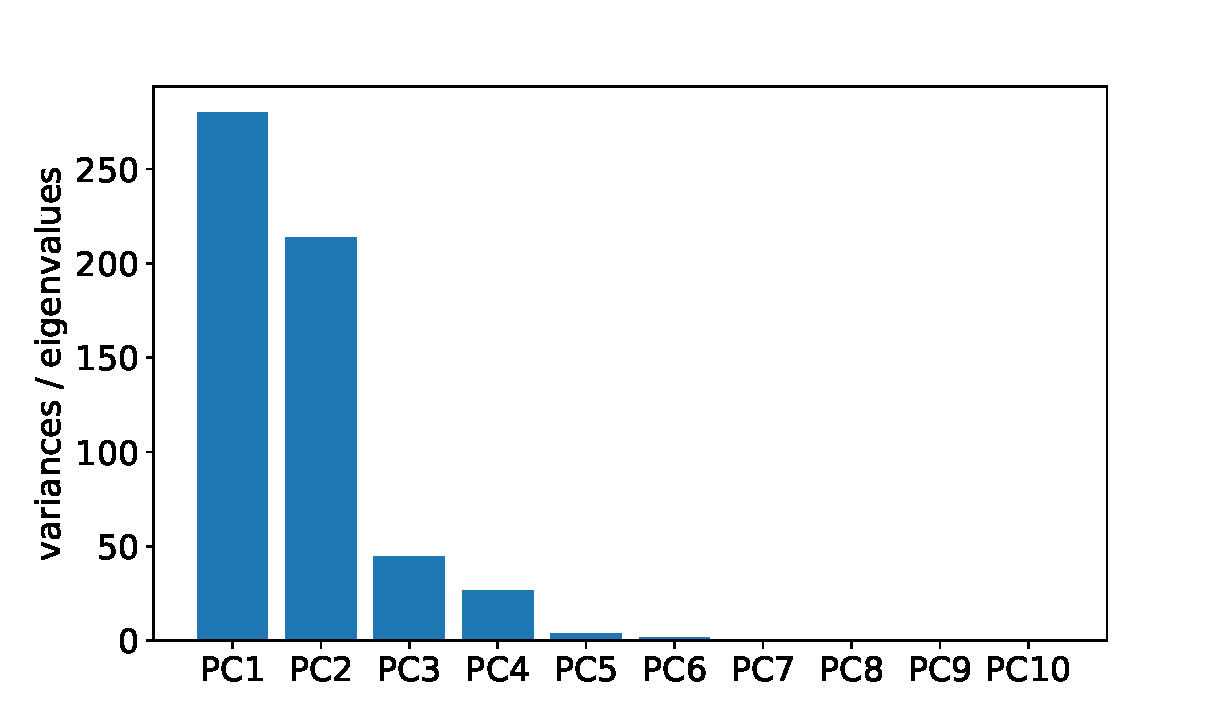
\includegraphics[width=0.6\textwidth]{img/screeplot_kpca_poly_d3}%
\captionof{figure}{Example of a scree plot}
\end{center}

\end{frame}

\subsection{Projection and Reconstruction error}

\begin{frame}\frametitle{How much better is this vs. simple trunctation?}
%\newpage

\only<1,2>{
The transformation onto the PCs is linear:
\begin{equation}
	\vec{x}_{\mathit{centered}} = \underbrace{ a_1 }_{ \vec{e}_1^\top \vec{x} } \vec{e}_1
		+ \underbrace{ a_2 }_{ \vec{e}_2^\top \vec{x} } \vec{e}_2
		+ \ldots
		+ \underbrace{ a_N }_{ \vec{e}_N^\top \vec{x} } \vec{e}_N
\end{equation}

Therefore, we can perfectly reconstruct observations by projecting them from PC space (i.e. feature space) back to the input space. \\
If we only use the \textcolor{red}{first} ${\color{red}M}$ PCs for reconstructing the observations, we will accumulate error.

\svspace{-5mm}

\begin{equation}
\widetilde{\vec{x}} = a_1 \vec{e}_1 + a_2 \vec{e}_2 + \ldots
		+ a_M \vec{e}_M
\end{equation}
}
		
\notesonly{We measure MSE between original centered observations and their corresponding reconstructions just as we did in \eqref{eq:mse}.}

\pause

\only<2,3>{
\begin{equation}
E = \frac{1}{p} \sum_{\alpha = 1}^{p} (\vec x_{\mathit{centered}} - \widetilde{\vec{x}})^2 = \frac{1}{p} \sum_{\alpha = 1}^{p} \sum_{j = M+1}^{N} (a_j^{(\alpha)})^2
\end{equation}
The MSE is equal to the sum of variances of the final $N-(M+1)+1$ components of the \emph{transformed} observations.\\
}
\only<3>{\notesonly{Since the PCs are ordered w.r.t to variance in descending order, }the variances of the last $N-M$ components of the transformed data are smallest.
The transformation is therefore optimal in the sense of minimal MSE.
}

\end{frame}

\mode*

\clearpage

%\section{References}
%\begin{frame}[allowframebreaks] \frametitle{References}
	%\scriptsize
	%\bibliographystyle{plainnat}
	%\bibliography{bibliography}
%\end{frame}

\end{rightcolumn}
\end{paracol}

\end{document}
